\documentclass{article}
%%%%%%%%%%%%%
% Loads packages
%%%%%%%%%%%%%
\usepackage[table]{xcolor}
\usepackage[utf8]{inputenc}
\usepackage[colorlinks=true,linkcolor=blue]{hyperref}
\usepackage{geometry} %package needed to set margins
\usepackage{fancyhdr}
\usepackage{graphicx}
\usepackage{amsmath}
\usepackage{amsthm}
\usepackage{mdframed}
\usepackage{tikz}
\usetikzlibrary{arrows.meta}
\usetikzlibrary{decorations.markings}
\usepackage{amsfonts}
\usepackage{wasysym}

\usepackage{listings}% http://ctan.org/pkg/listings
\lstset{
  basicstyle=\ttfamily,
  mathescape
}


\pagestyle{fancy}
\fancyhf{}
\chead{\textbf{Homework 11}}
\lhead{Math 213, Fall 2024}
\rhead{Due Sunday, 12/8 at 11:59pm}

%%%%%%%%%%%%%
% Sets margins
%%%%%%%%%%%%%
\newgeometry{left=1.5in,right=1in,top=1in,bottom=1in}
\setlength\headsep{3pt}

%%%%%%%%%%%%%
% Creates problem and solution environments
%%%%%%%%%%%%%

% Solution Environment
\newenvironment{solution}{\begin{proof}[Solution]}{\end{proof}}

% Problem Environment
\newenvironment{problem}[1]
    {\begin{mdframed}[default]
    \textbf{Problem #1:}
    }
    {\end{mdframed}
    }
    
%%%%%%%%%%%
% Custom Commands
%%%%%%%%%%%
\newcommand{\gOne}{\cellcolor{green!50!white} 1}
\newcommand{\rZero}{\cellcolor{red!50!white} 0}

\begin{document}

\begin{problem}{\S 10.6 - 3}
Find the length of a shortest path between $a$ and $z$ in the given weighted graph.

\begin{center}
    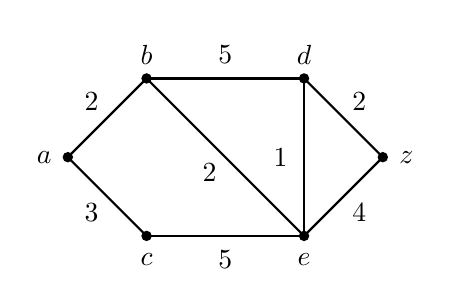
\begin{tikzpicture}
    \coordinate (a) at (0,0);
    \coordinate (b) at (1,1);
    \coordinate (c) at (1,-1);
    \coordinate (d) at (3,1);
    \coordinate (e) at (3,-1);
    \coordinate (z) at (4,0);
    \begin{scope}[thick]
            
            % draws vertices
            \node[circle, fill=black,scale = 0.4] at (a){};
            \node[circle, fill=black,scale = 0.4] at (b){};
            \node[circle, fill=black,scale = 0.4] at (c){};
            \node[circle, fill=black,scale = 0.4] at (d){};
            \node[circle, fill=black,scale = 0.4] at (e){};
            \node[circle, fill=black,scale = 0.4] at (z){};
            
            % labels vertices
            \node at (-0.3,0) {$a$};
            \node at (1,1.3) {$b$};
            \node at (1,-1.3) {$c$};
            \node at (3,1.3) {$d$};
            \node at (3,-1.3) {$e$};
            \node at (4.3,0) {$z$};
            
            % draws edges
            \draw[postaction={decorate}] (a) to (b);
            \draw[postaction={decorate}] (b) to (d);
            \draw[postaction={decorate}] (d) to (z);
            \draw[postaction={decorate}] (z) to (e);
            \draw[postaction={decorate}] (e) to (c);
            \draw[postaction={decorate}] (c) to (a);
            \draw[postaction={decorate}] (b) to (e);
            \draw[postaction={decorate}] (d) to (e);

            % labels edges
            \node at (0.3,0.7) {$2$};
            \node at (0.3,-0.7) {$3$};
            \node at (2,1.3) {$5$};
            \node at (2,-1.3) {$5$};
            \node at (1.8,-0.2) {$2$};
            \node at (2.7,0) {$1$};
            \node at (3.7,0.7) {$2$};
            \node at (3.7,-0.7) {$4$};
            \end{scope}
    \end{tikzpicture}
\end{center}
\end{problem}

\begin{problem}{\S 10.6 - 5}
Find a shortest path between $a$ and $z$ in the weighted graph in Exercise~3.
\end{problem}

\begin{problem}{\S 10.6 - 6}
Find the length of a shortest path between these pairs of
vertices in the weighted graph in Exercise 3.

\begin{enumerate}
    \item[(a)] $a$ and $d$
    \item[(d)] $b$ and $z$
\end{enumerate}
\end{problem}

\begin{problem}{\S 10.6 - 7}
Find shortest paths in the weighted graph in Exercise 3
between the pairs of vertices in Exercise 6 (parts a and d).
\end{problem}

\begin{problem}{\S 10.6 - 26}
Solve the traveling salesperson problem for this graph
by finding the total weight of all Hamilton circuits and
determining a circuit with minimum total weight.

\begin{center}
    \begin{tikzpicture}
    \coordinate (a) at (1,2);
    \coordinate (b) at (3,2);
    \coordinate (c) at (4,0);
    \coordinate (d) at (2,-1);
    \coordinate (e) at (0,0);
    \begin{scope}[thick]
            
            % draws vertices
            \node[circle, fill=black,scale = 0.4] at (a){};
            \node[circle, fill=black,scale = 0.4] at (b){};
            \node[circle, fill=black,scale = 0.4] at (c){};
            \node[circle, fill=black,scale = 0.4] at (d){};
            \node[circle, fill=black,scale = 0.4] at (e){};
            \node[circle, fill=black,scale = 0.4] at (z){};
            
            % labels vertices
            \node at (0.8,2.2) {$a$};
            \node at (3.2,2.2) {$b$};
            \node at (4.3,0) {$c$};
            \node at (2,-1.3) {$d$};
            \node at (-0.3,0) {$e$};
            
            % draws edges
            \draw[postaction={decorate}] (a) to (b);
            \draw[postaction={decorate}] (a) to (c);
            \draw[postaction={decorate}] (a) to (d);
            \draw[postaction={decorate}] (a) to (e);
            \draw[postaction={decorate}] (b) to (c);
            \draw[postaction={decorate}] (b) to (d);
            \draw[postaction={decorate}] (b) to (e);
            \draw[postaction={decorate}] (c) to (d);
            \draw[postaction={decorate}] (c) to (e);
            \draw[postaction={decorate}] (d) to (e);

            % labels edges
            \node at (0.3,1) {$7$};
            \node at (2,2.2) {$3$};
            \node at (3.7,1) {$10$};
            \node at (3,-0.7) {$6$};
            \node at (1,-0.7) {$1$};
            \node at (1,0.2) {$5$};
            \node at (0.9,0.8) {$2$};
            \node at (3.1,0.8) {$8$};
            \node at (1.7,0.5) {$4$};
            \node at (2.3,0.5) {$9$};
            \end{scope}
    \end{tikzpicture}
\end{center}
\end{problem}

\begin{problem}{\S 10.7 - 6}
Determine whether the given graph is planar.
If so, draw it so that no edges cross.

\begin{center}
    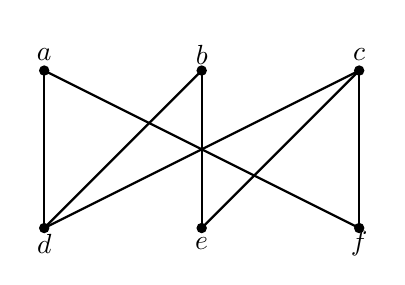
\begin{tikzpicture}
    \coordinate (a) at (0,2);
    \coordinate (b) at (2,2);
    \coordinate (c) at (4,2);
    \coordinate (d) at (0,0);
    \coordinate (e) at (2,0);
    \coordinate (f) at (4,0);
    \begin{scope}[thick]
            
            % draws vertices
            \node[circle, fill=black,scale = 0.4] at (a){};
            \node[circle, fill=black,scale = 0.4] at (b){};
            \node[circle, fill=black,scale = 0.4] at (c){};
            \node[circle, fill=black,scale = 0.4] at (d){};
            \node[circle, fill=black,scale = 0.4] at (e){};
            \node[circle, fill=black,scale = 0.4] at (f){};
            
            % labels vertices
            \node at (0,2.2) {$a$};
            \node at (2,2.2) {$b$};
            \node at (4,2.2) {$c$};
            \node at (0,-0.2) {$d$};
            \node at (2,-0.2) {$e$};
            \node at (4,-0.2) {$f$};
            
            % draws edges
            \draw[postaction={decorate}] (a) to (d);
            \draw[postaction={decorate}] (a) to (f);
            \draw[postaction={decorate}] (b) to (d);
            \draw[postaction={decorate}] (b) to (e);
            \draw[postaction={decorate}] (c) to (d);
            \draw[postaction={decorate}] (c) to (e);
            \draw[postaction={decorate}] (c) to (f);
            \end{scope}
    \end{tikzpicture}
\end{center}
\end{problem}

\begin{problem}{\S 10.7 - 11}
Show that $K_5$ is nonplanar using an argument similar to that given in Example 3.
\end{problem}

\begin{problem}{\S 10.7 - 13}
Suppose that a connected planar graph has six vertices, each of degree four. Into how many regions is the plane divided by a planar representation of this graph?
\end{problem}

\begin{problem}{\S 10.7 - 14}
Suppose that a connected planar graph has $30$ edges. If a planar representation of this graph divides the plane into $20$ regions, how many vertices does this graph have?
\end{problem}

\begin{problem}{\S 10.8 - 1}
Construct the dual graph for the map shown. (See Rosen for the map!) Then find the number of colors needed to color the map so that no two adjacent regions have the same color.
\end{problem}

\begin{problem}{\S 10.8 - 5}
Find the chromatic number of the given graph.

\begin{center}
    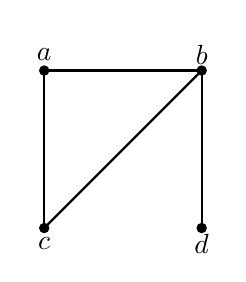
\begin{tikzpicture}
    \coordinate (a) at (0,2);
    \coordinate (b) at (2,2);
    \coordinate (c) at (0,0);
    \coordinate (d) at (2,0);
    \begin{scope}[thick]
            
            % draws vertices
            \node[circle, fill=black,scale = 0.4] at (a){};
            \node[circle, fill=black,scale = 0.4] at (b){};
            \node[circle, fill=black,scale = 0.4] at (c){};
            \node[circle, fill=black,scale = 0.4] at (d){};
            
            % labels vertices
            \node at (0,2.2) {$a$};
            \node at (2,2.2) {$b$};
            \node at (0,-0.2) {$c$};
            \node at (2,-0.2) {$d$};
            
            % draws edges
            \draw[postaction={decorate}] (a) to (b);
            \draw[postaction={decorate}] (a) to (c);
            \draw[postaction={decorate}] (b) to (c);
            \draw[postaction={decorate}] (b) to (d);
            \end{scope}
    \end{tikzpicture}
\end{center}
\end{problem}

\begin{problem}{\S 10.8 - 6}
Find the chromatic number of the given graph.

\begin{center}
    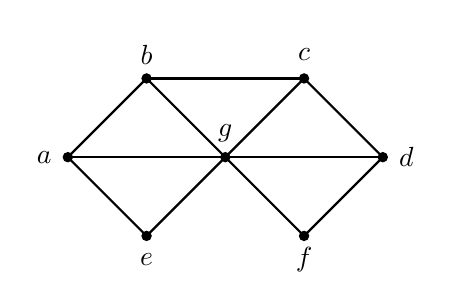
\begin{tikzpicture}
    \coordinate (a) at (0,0);
    \coordinate (b) at (1,1);
    \coordinate (c) at (3,1);
    \coordinate (d) at (4,0);
    \coordinate (e) at (3,-1);
    \coordinate (f) at (1,-1);
    \coordinate (g) at (2,0);
    \begin{scope}[thick]
            
            % draws vertices
            \node[circle, fill=black,scale = 0.4] at (a){};
            \node[circle, fill=black,scale = 0.4] at (b){};
            \node[circle, fill=black,scale = 0.4] at (c){};
            \node[circle, fill=black,scale = 0.4] at (d){};
            \node[circle, fill=black,scale = 0.4] at (e){};
            \node[circle, fill=black,scale = 0.4] at (f){};
            \node[circle, fill=black,scale = 0.4] at (g){};
            
            % labels vertices
            \node at (-0.3,0) {$a$};
            \node at (1,1.3) {$b$};
            \node at (3,1.3) {$c$};
            \node at (4.3,0) {$d$};
            \node at (1,-1.3) {$e$};
            \node at (3,-1.3) {$f$};
            \node at (2,0.3) {$g$};
            
            % draws edges
            \draw[postaction={decorate}] (a) to (b);
            \draw[postaction={decorate}] (b) to (c);
            \draw[postaction={decorate}] (c) to (d);
            \draw[postaction={decorate}] (d) to (e);
            \draw[postaction={decorate}] (f) to (a);
            \draw[postaction={decorate}] (a) to (g);
            \draw[postaction={decorate}] (b) to (g);
            \draw[postaction={decorate}] (c) to (g);
            \draw[postaction={decorate}] (d) to (g);
            \draw[postaction={decorate}] (e) to (g);
            \draw[postaction={decorate}] (f) to (g);
            \end{scope}
    \end{tikzpicture}
\end{center}
\end{problem}

\begin{problem}{\S 10.8 - 15}
What is the chromatic number of $W_n$?
\end{problem}

\begin{problem}{\S 10.8 - 16}
Show that a simple graph that has a circuit with an odd
number of vertices in it cannot be colored using two colors.
\end{problem}

\end{document}